% Før første subseksjon: ; 2.1.3: Nøkkel-verdi-lagre; 2.1.4: Dokumentlagre; 2.1.5: KFL; 2.1.2 Ett eget overordnet kapittel om aggregatorientering; 2.1.1 mySQL?
% 2.1 - Om relasjonelle modeller, motivasjonen bak NoSQL
\section{Den relasjonelle datamodellen}

% Den relasjonelle datamodellen, i.e. MariaDB og Postgres (Bøyningen av sybstantivet 'tuppel' samsvarer med Bratsbergengens skrivemåte i hans artikkel om relasjonsdatabaser hos SNL)
For å forstå framveksten av NoSQL - databaser er . I den relasjonelle datamodellen organiseres forskjellige former for applikasjonsdata inn i relasjoner, og data tilhørende samme relasjon inndeles i atomiske, disjunkte enheter kalt \emph{tupler}. En tuppel er en flat, endimensjonal liste av dataverdier. Hver av disse verdiene korresponderer til nøyaktig ett attributt av relasjonen tuppelen er lagret i.

% Strukturelle begrensninger i relasjonsdatabaser
Det foreligger visse begrensninger på denne datastrukturen. Til eksempel kan ikke en enkelt tuppel nøstes inn i en annen, og hvert attributt i tuppelen har én atomisk korresponderende verdi, aldri en liste av verdier. Nå skal det sies at nyere versjoner av MariaDB støtter JSON-objekter som datatype \citep{mariadb}. JSON-objekter er serialiserte (dsv objekter konverterte til strenger), fleksible dataenheter som kan inneholde nøstede datastrukturer.

Imidlertid har ikke databasesystemet noen forståelse for de enkelte dataelementer som objektet innkapsler, det ser bare en helhetlig, ugjennomsiktlig dataenhet, nemlig verdien av ett attributt i relasjonen. Ettersom tupler er den minste, udelelige dataenheten i den relasjonelle modellen er det korrekt å fastslå at spørringer opererer med og returnerer (et helt antall) tupler for hver enkelt spørring \citep{sadalage2013}. Riktignok går det an å utvelge distinkte attributter i spørringen, også kjent som kommandoen \texttt{PROJECT} i relasjonell algebra, likefullt er den tellbare dataenheten i resultantrelasjonen tupler, også referert til som rader i kontekst av databaseapplikasjoner.

% Spørringsfleksibilitet (JOIN + avanserte operasjoner) - Fra databasepensum
Følgelig gir slike strengt strukturerte datamodeller stor fleksibilitet for spørringene som utføres av databasesystemet. Det kan for eksempel samle sammen alle verdier for ett spesifikt numerisk attributt i én bestemt relasjon, summere disse  attributtverdiene sammen og returnere resultatet som et separat attributt i resultanttuppelen. På samme vis kan relasjonsdatabasesystemet kalkulere gjennomsnittet for alle eller enkelte av tuplene i en relasjon, telle opp antallet tupler i den, finne den høyeste numeriske verdien eller finne den laveste.

Ved hjelp av JOIN-operasjoner finner man eksisterende tupler fra forskjellige relasjoner, relatert til hverandre via fremmednøkler, og resultanten av JOINen kan systemet også kalle disse aggregeringsoperasjonene på. NoSQL - databaser har ikke den samme fleksibiliteten til selv å utføre slike spørreoperasjoner: Hver spørring henter kun én dataenhet ad gangen, noe som holder især for nøkkelverdilagre. Hver spørring er logisk sett bare et oppslag på en nøkkel i en hashtabell. Eventuell aggregering der sum, gjennomsnitt eller ekstremalverdier regnes må gjøres i selve applikasjonen, etter at oppslag på \textbf{samtlige} nøkler er gjort i databasen.

% Figur 1
\begin{figure}[ht]
    \centering
    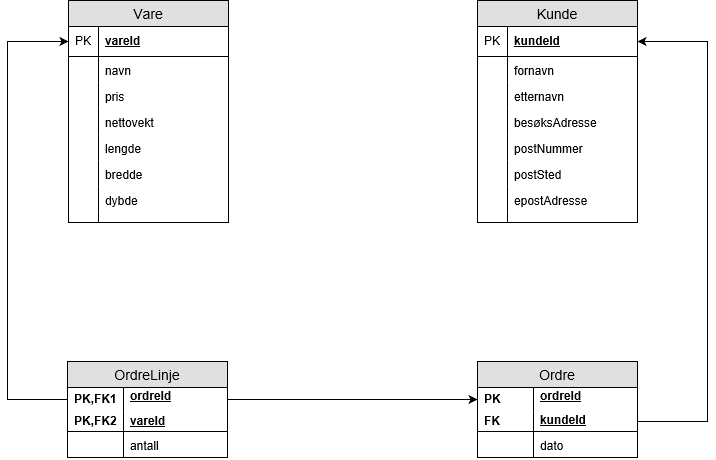
\includegraphics{fig/NettbutikkOrdreModell.png}
    \caption{Diagram over tabeller i en relasjonsdatabase som registrerer ordrer fra kunder i en netthandelapplikasjon.}
    \label{fig1}
\end{figure}
 
\subsection{Impedansproblemet (Impedance mismatch problem)}

I en typisk netthandelapplikasjon er applikasjonens datamodell denotert i form av dataobjekter midlertidig lagret i primærminnet, mer presist sagt, i adresseområdet til èn, eller flere, av nettleserens kjørende prosesser i kundens datamaskin. Variablene i datafeltene i disse objektene kan være saå mangt: strenger, tall, referenser til andre objekter, lister bestående av ovennevnte typer. Disse dataobjektene endres i sanntid av kunden som aksesserer nettbutikken gjennom standardiserte interaksjonselementer som tekstfelt, knapper, slidere, sjekkbokser og radiobokser, gruppert sammen i dynamiske sideelementer kjent som skjema (eng. ''form''). Et praktisk eksempel på et skjema i en netthandel er handlevognen, som viser kunden hvilke vareartikler han (foreløpig) vil kjøpe, hvor mange av hver vare som ''ligger'' i handlevogna, og hvor mye varene koster sammenlagt.

Når det kommer til å skrive dataene fra web-skjemaet til disk i en relasjonsdatabase ser ting annerledes ut. Her persisteres data om varer (navn, identifikasjonsnummer, størrelsesdimensjoner, nettovekt, og enhetspris \footnote{Gitt at hver enkelt vare-tuppel representerer en diskret enhet, til eksempel én bøtte maling eller én sekk med poteter}) til en egen relasjon. En annen relasjon holder data om kunder, en tredje holder på informasjon om bestillinger, og for normaliseringens skyld eksisterer en egen jointabell kalt Ordrelinje som kopler sammen Ordre og Vare, som illustrert i tabell-diagrammet i \ref{fig1}. Denne uoverensstemmelsen mellom strukteren av applikasjonsdata i programminne og strukturen på de samme dataene i en relasjonsdatabase refereres til i industrien som ''the impedance mismatch'' \citep{sadalage2013}.

Følgelig må applikasjonsutviklere konvertere data fra spørringsresultater til den dataobjektstrukturen applikasjonen påkrever, noe som per idag ofte løses ved å innføre et seperat abstrahert lag i applikasjonens logiske arkitektur: En tredjepartsmodul kalt ''object-relational mapper'' (ORM). For språket Java kan man bruke Hibernate\footnote{\url{http://hibernate.org/orm/}}, JavaScript har SequelizeJS\footnote{\url{http://docs.sequelizejs.com/}}, og PHP-utviklere kan bruke Doctrine\footnote{\url{http://www.doctrine-project.org/}}, som også er en del av webapplikasjonsrammeverket Symfony\footnote{\url{http://symfony.com/}}. Med slike tredjepartsbibliotek følger selvfølgelig et nytt mønster som utviklere blir nødt til å forholde seg skal de ta det i bruk. Ettersom det relasjonelle datalaget abstraheres bort er det tilforlatelig å ''glemme'' at applikasjonsdata faktisk persisteres i en relasjonell database. En tilsynelatende enkel henteoperasjon på objektform kan fort translatere til to kostbare JOIN-operasjoner i databasen som kjøres hver gang spørringen utføres.

% Distribuering av data utover flere instanser == katastrofe
En annen innvending mot den relasjonelle datamodellen involverer hvordan den støtter skalering av arbeidslast med hensyn på økende antall brukere, økende antall datakilder, og økende spørringsfrekvens databasesystemet utsettes for. Datamodellen ble etablert på 70-tallet, i en æra lenge før distribuert databeregning tok av i bedriftsmarkedet. Relasjonsdatabaser er designet med tanke på monolittiske systemarkitekturer, programvarearkitekturer hvis system kjører på én enkel datamaskin, fordelt på et sett med prosesser innad i den. For et begrenset antall datakilder/brukere er slike systemer i noen grad vertikalt skalerbare, det vil si at økt last på systemet kan løses ved å oppgradere maskinvaren. Denne metoden er innlysende nok kostbar i det lange løp ettersom maskinvare som skiftes ut ikke er brukelig for systemet lengre. Da er det billigere å skalere horisontalt, det vil si å kjøre programvaresystemet i en klynge av datamaskiner sammenkoplet over et IP - nettverk. Hver av disse datamaskinene er billige, altså består de av maskinvarekomponenter som yter dårligere enn den jevne stordatamaskin som prosesserer banktransaksjoner.  Som demonstrert i følgende eksempel statuert av \cite{george2011} skal vi se at å operere i klynget system ikke er så lett når data modelleres relasjonelt.

% Jamfør HBase - penusm i TDT4150
\subsection{Hush}

Hush er en (fiktiv) url-forkortelsestjeneste som i begynnelsen har omtrent et par tusen brukere, og vedlikeholdes og bygges med gratis tredjepartsmoduler, blant annet driftes en LAMP-tjener (Linux, Apache, MariaDB, PHP) som leverer en prototype av denne tjenesten i form av en webapplikasjon. Hush sin relasjonelle databasemodell normaliserer sine data ved å definere fire tabeller, \texttt{user}, \texttt{url}, \texttt{shorturl}, og \texttt{click} \citep{george2011}. De tre sistnevnte tabellene er assosiert med \texttt{user} gjennom en fremmednøkkel som refererer til nøkkelattributtet til den tabellen. I tillegg er brukertabellen og kort-URL-tabellen indeksert etter sine respektive nøkkelattributter for å gjøre oppslag på korte URLer og brukere raskere. Ved å sluse endringer inn i systemet som transaksjoner sikrer man at de relaterte tabellene (den for URLer, korte URLer og klikk) endres sekvensielt og fullstendig uavhengig av hvor samtidig de uavhengige skriveoperajsonene forekommer slik at et strengt konsistensnivå opprettholdes tuplene imellom.

Transaksjoner er en velprøvd og høyt akseptert logisk modell for databehandling. Relasjonelle databaser tillater oppdatering av eller lesing av tupler i opptil flere relasjoner innen et sett med atomiske operasjoner. Det er den enkelte mengden av hendelser som heter for en transaksjon. En transaksjon avgrenser mengden av hendelser og skriver enten samtlige eller ingen endringer til disk.

Transaksjonenes egenskaper beskrives med akronymet ACID: De er atomiske, dvs at samtlige hendelser i transaksjonen blir enten gjennomført fullstendig eller ei; konsistente (eng. ''Consistent''), dvs at to transaksjoner som kjører parallellt alltid medfører det samme sluttresultatet; isolerte, det vil si holdbare i den grad transaksjonen persisteres til disk (eng. ''Durable''). Transaksjonsmodellen fremmer en spesifikk handling, \texttt{COMMIT}, som signaliserer at endringene spesifisert i den enkelte transaksjon er blitt gjort permanente.

Denne monolittiske databasearkitekturen fungerer med det gitte antall brukere. Idet tjenesten blir verdenskjent, og antallet brukere øker eksponensielt med fire tierpotenser, blir arbeidslasten for databasetjeneren etter hvert for stor å handtere alene. Den naturlige løsningen på å tekkes vekstraten i databasens arbeidslast er å innføre flere databasetjenere installert på separate datamaskiner. Når skriveoperajsoner og leseoperasjoner i et databasesystem distribueres utover en klynge tjenere, er det viktig å organisere dem slik at arbeidslasten av skrivinger og lesinger jevnfordeles metodisk slik at databasesystemets distribuerte natur ikke er synlig for applikasjonen som utfører spørringen. En vanlig organiseringsmetode er master-slave-replikering, der én master-tjener mottar alle skriveoperasjoner for å serialisere dem \citep{george2011}.

I historien om Hush er dette veien dets utviklere tar: Slavetjenerne får motta lesespørringer, én enkel mastertjener fordeler skriveoperasjoner blant slavene. Hush er en applikasjon der leseoperasjoner utnummerer skriveoperasjoner i antall, det hender jo oftere at noen klikker på en frokortet lenke snarere enn at noen poster en lenkeforkortelse på tjenesten. For en stakket fungerer denne lastfordelingen utover klyngen, men etterhvert er tilveksten av brukere såpass stor at leseoperasjonene samlet sett blir trege. Etter hvert blir også masterdatabasetjeneren som handterer samtlige skriveoperasjoner blir en flaskehals i systemet \citep{george2011}.

For å øke ytelsen til leseoperasjonen installerer utviklerne av Hush et distribuert hurtiglager med det minnebaserte nøkkelverdilageret Memcached\footnote{\url{https://www.memcached.org/}}. Imidlertid svekkes oppdateringskonsistensnivået til systemet ettersom dataverdier i hurtiglageret må skiftes ut etter hvert som transaksjoner behandles av mastertjeneren. For å holde tritt med den økende skrivelasten kunne man oppgradere mastertjenerens maskinvare, altså å skalere oppover, en lite bærekraftig løsning i lengden ettersom det finnes et øvre fysisk tak på antallet mikrotransistorer som kan få plass innen én kvadratmillimeter mikrochip. Det er også en svært kostbar, fordi slavetjenernes maskinvare må nødvendigvis også oppgraderes i lengden for å holde tritt med de stadig innkommende skriveforespørslene fra mastertjeneren. På toppen av disse bekymringene går også utførelse av JOIN - operasjonene for tregt for at systemene skal kunne holde tritt med den økende frekvensen av spørringer fra applikasjonstjenerne, så man velger da å denormalisere tabellene. Det er nå kommet tydelig fram at den relasjonelle datamodellen nå er til mer bry enn den er til hjelp for Hush-utviklerne.

Av denne historien kan man oppsummere at relasjonelle databasesytemer ikke er laget for å kjøre i et distribuert miljø. Ei heller lar de seg skaleres horisontalt, altså at løsningen på økende arbeidslast er å legge til en datamaskin med billige maskinvarekomponenter i et distribuert nettverk av andre liknende datamaskiner og jevnfordele spørringene utover dem. En relasjonsdatabasetjener kan istedet skaleres vertikalt, det vil si at prosessorenheter med høyere klokkefrekvenser og minnekort og harddisker med større datakapasitet installeres i tjenermaskinen og erstatter de gamle. Ikke bare er dette en utålelig dyr løsning, men den forårsaker også i vedlikeholdsperioder, dog bytte av maskin i dag tar stadig kortere tid hos dagens skytjenester, der appliakjsonen ikke kan betjene noen brukerforespørsler. For å takle lagring og behandling av stadig større datavolum, må vi se nærmere på en annen, nyere og mer fleksibel måte å strukturere lagret data på. 

